\chapter{Química bioinorgánica}\label{ch:b3:bioinorganic}

Nuestra sangre es roja a causa del hierro; la sangre de un cangrejo herradura es incolora en
sus venas y se vuelve azul al aire, porque transporta el oxígeno sobre cobre. La vida usa
un puñado de iones metálicos para las tareas que ningún grupo orgánico puede hacer: unir el oxígeno
de forma reversible, mover electrones de uno en uno, romper el agua, reducir el nitrógeno,
volver una molécula de agua lo bastante ácida para atacar el dióxido de carbono. Este capítulo
lee esas tareas con las herramientas de la química de coordinación: \omterm{def:b3:bioinorganic:hsab}{ácidos duros} y
blandos, campos de ligandos y estados de espín, equilibrios y leyes de velocidad, y termina
con los metales usados como fármacos.

\begin{recall}
El volumen del segundo año trató los $\alpha$-aminoácidos, las cadenas laterales y los péptidos, las bases nitrogenadas
y los nucleótidos, los complejos de coordinación, los campos de ligandos, el alto y el bajo espín, y
los nucleófilos y electrófilos duros y blandos; el volumen del primer año, las constantes de
complejación y la escala pL. Los \cref{ch:b3:complex-spectra-magnetism} y
\cref{ch:b3:complex-mechanisms} dieron los espectros, la teoría de Marcus y la acuación del
cisplatino; el \cref{ch:b3:complex-kinetics}, la cinética de Michaelis--Menten, y
el \cref{ch:b3:advanced-nmr}, el tiempo de relajación $T_1$.
\end{recall}

\begin{omfigure}
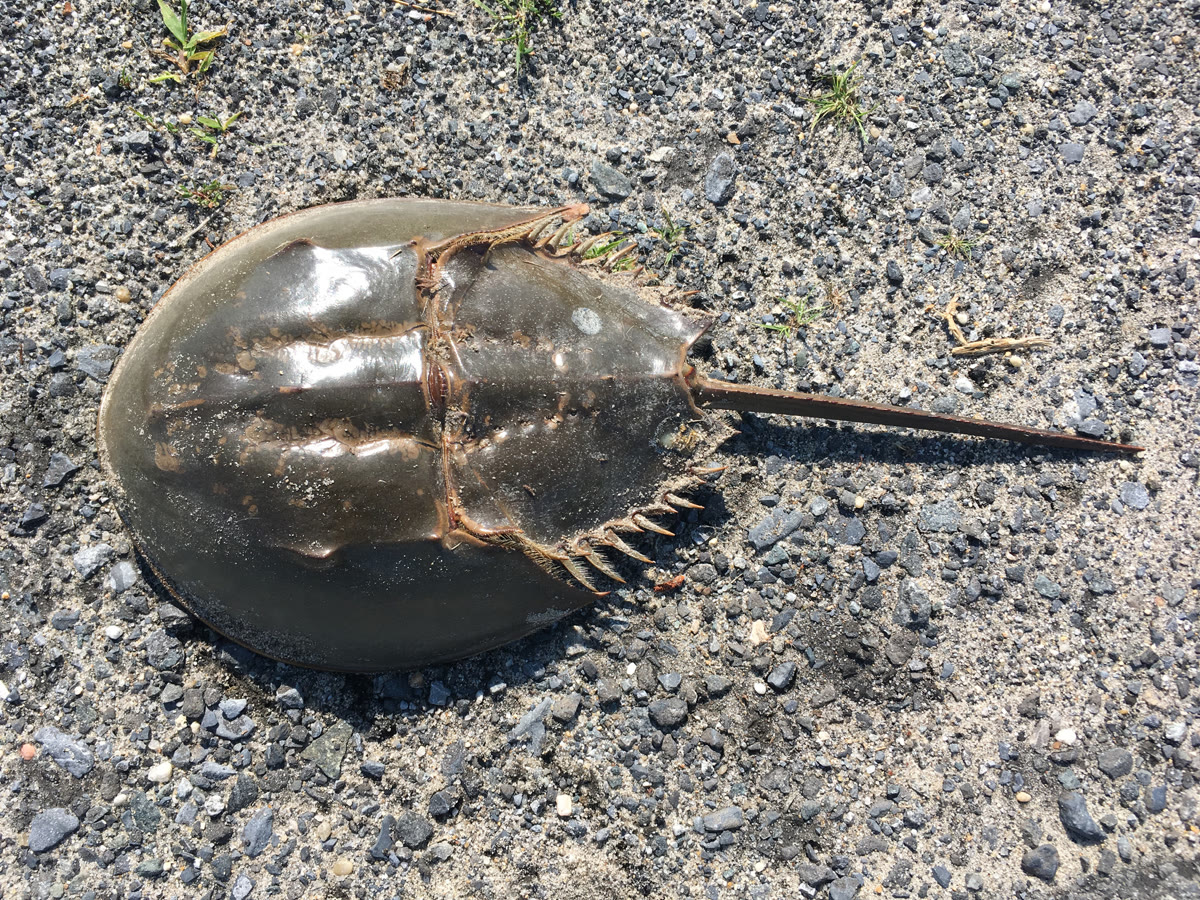
\includegraphics[width=0.5\linewidth]{images/book4/horseshoe-crab.jpg}

{\small Un cangrejo herradura del Atlántico. Su sangre transporta el oxígeno sobre la hemocianina, una
proteína de cobre, y es azul cuando está oxigenada. Fotografía: Kaldari, CC0.}
\end{omfigure}

\section{Los metales en biología}

\begin{definition}[Metaloproteínas]\label{def:b3:bioinorganic:metalloprotein}
Una \emph{metaloproteína}\index{metaloproteina@metaloproteína} es una proteína que contiene
iones metálicos unidos; una \emph{metaloenzima}\index{metaloenzima} es una metaloproteína que
cataliza una reacción. Un \emph{cofactor}\index{cofactor} es una especie no proteica,
un ion metálico o una molécula pequeña, unida a una proteína y necesaria para su
actividad.
\end{definition}

Los metales que importan en cantidad son el sodio, el potasio, el magnesio y el
calcio, que sobre todo transportan carga y sostienen estructuras; los metales de transición
hierro, cinc, cobre, manganeso, cobalto, molibdeno y níquel aparecen en trazas,
pero llevan buena parte de la química. Una proteína elige su metal mediante los átomos
dadores que ofrece y su geometría.

\begin{definition}[Ácidos duros y blandos]\label{def:b3:bioinorganic:hsab}
Un \emph{ácido duro}\index{acido duro@ácido duro} es un ácido de Lewis pequeño, muy cargado y poco
polarizable ($\ce{H+}$, $\ce{Mg^2+}$, $\ce{Ca^2+}$, $\ce{Fe^3+}$); un \emph{ácido
blando}\index{acido blando@ácido blando} es uno grande, polarizable y de carga baja ($\ce{Cu+}$, $\ce{Ag+}$,
$\ce{Hg^2+}$, $\ce{Cd^2+}$). El \emph{principio de los ácidos y bases duros y blandos}\index{principio de los acidos y bases duros y blandos@principio de los ácidos y bases duros y blandos}
establece que los ácidos duros se unen preferentemente a las bases duras
(dadores de oxígeno, fluoruro) y los ácidos blandos a las bases blandas (dadores de azufre, yoduro).
\end{definition}

En las proteínas, los carboxilatos y los fenolatos son duros, el tiolato de la cisteína y
el tioéter de la metionina, blandos, y el imidazol de la histidina, intermedio. El hierro(III)
se sitúa entre dadores de oxígeno, el cobre(I) entre dadores de azufre, y el cinc, un ácido
intermedio, con histidina y cisteína; el mercurio y el cadmio son tóxicos en parte
porque secuestran las cisteínas de las \omterm{def:b3:complex-kinetics:enzyme}{enzimas}.

\begin{definition}[Serie de Irving--Williams]\label{def:b3:bioinorganic:irving-williams}
La \emph{serie de Irving--Williams}\index{serie de Irving--Williams} es el orden
de estabilidad de los complejos de alto espín de los iones divalentes de la primera
serie de transición con un ligando dado:
$\ce{Mn^2+} < \ce{Fe^2+} < \ce{Co^2+} < \ce{Ni^2+} < \ce{Cu^2+} > \ce{Zn^2+}$.
\end{definition}

\begin{proposition}[Orden de Irving--Williams]\label{prop:b3:bioinorganic:irving-williams}
La serie se cumple para casi todos los ligandos (una observación experimental); sigue
la disminución del radio iónico del manganeso al cobre, la energía de estabilización
del campo de ligandos, nula para $d^5$ y máxima para $d^8$, y la distorsión
de Jahn--Teller del cobre(II), que acorta cuatro de sus enlaces.
\end{proposition}

\begin{proof}[Argumento]
El radio disminuye a lo largo de la fila a medida que crece la carga nuclear, lo que refuerza
la atracción electrostática de todo ligando. La estabilización del campo de ligandos de los
iones octaédricos de alto espín (\cref{ch:b3:complex-spectra-magnetism}) es $0$, $4$,
$8$, $12$ y $6\,\mathrm{Dq}$ para $d^5$ a $d^9$, y $0$ para $d^{10}$: se suma a la tendencia hasta el níquel y
cae para el cinc; el cobre(II) recupera más de lo que sugiere su estabilización gracias a
su distorsión tetragonal, que da cuatro enlaces cortos y fuertes.
\end{proof}

Una consecuencia que las células deben gestionar: el cobre y el cinc desplazarían a los
demás iones de la mayoría de los sitios, de modo que sus concentraciones libres se mantienen extremadamente bajas
mediante proteínas transportadoras específicas.

\section{El transporte del oxígeno}

\begin{definition}[Porfirinas y hemo]\label{def:b3:bioinorganic:haem}
Una \emph{porfirina}\index{porfirina} es un macrociclo grande, plano y aromático de cuatro
anillos de pirrol unidos por puentes metino, cuyos cuatro nitrógenos se unen a un ion metálico
situado en su centro. El \emph{hemo}\index{hemo} es el complejo de hierro de la protoporfirina~IX,
el \omterm{def:b3:bioinorganic:metalloprotein}{cofactor} de la hemoglobina, la mioglobina y los citocromos.
\end{definition}

En la mioglobina y la hemoglobina, el hierro del \omterm{def:b3:bioinorganic:haem}{hemo} tiene un quinto ligando por debajo del
anillo, el nitrógeno de la histidina proximal, y una sexta posición libre para el $\ce{O2}$.
El hierro(II) desoxi es de alto espín: un electrón en el orbital $d_{x^2-y^2}$, que apunta hacia los cuatro
nitrógenos, lo hace demasiado grande para el hueco del anillo, y se sitúa fuera del
plano, hacia la histidina. Al unir el $\ce{O2}$ pasa a bajo espín, se hace más pequeño y
entra en el plano, arrastrando consigo la histidina y la hélice de la proteína.

\begin{omfigure}
% ledger: pdb:Hb.deoxy.FeN4, pdb:Hb.oxy.FeN4
\begin{tikzpicture}[font=\small, scale=0.9]
  \foreach \x/\lab/\dz/\oxy in {0/desoxi (alto espín)/-0.34/0, 6.4/oxi (bajo espín)/-0.04/1} {
    \begin{scope}[xshift=\x cm]
      \draw[omDef, line width=2.6pt] (-2.2,0) -- (2.2,0);
      \node[font=\scriptsize, anchor=west, omDef] at (2.3,0) {porfirina};
      \fill[omThm] (0,\dz*1.5) circle (0.22);
      \node[font=\scriptsize, anchor=north west] at (0.2,\dz*1.5-0.12) {Fe};
      \draw[black!70, line width=1pt] (0,\dz*1.5-0.22) -- (0,-1.55);
      \node[draw=black!70, regular polygon, regular polygon sides=5, minimum size=7mm, inner sep=0pt] at (0,-1.95) {};
      \node[font=\scriptsize, anchor=west] at (0.45,-1.95) {His proximal};
      \node[font=\small\bfseries] at (0,1.9) {\lab};
      \ifnum\oxy=1
        \draw[black!70, line width=1pt] (0,0.2) -- (0,0.85) -- (0.55,1.25);
        \fill[red!75] (0,0.85) circle (0.13) (0.55,1.25) circle (0.13);
        \node[font=\scriptsize, anchor=west] at (0.75,1.2) {$\ce{O2}$, angular};
      \fi
    \end{scope}
  }
  \draw[<->, black!60] (-1.0,0) -- (-1.0,-0.51) node[midway, left, font=\scriptsize] {\qty{0.34}{\angstrom}};
\end{tikzpicture}

{\small El hierro del \omterm{def:b3:bioinorganic:haem}{hemo} visto de perfil, con su desplazamiento respecto del anillo dibujado a
escala (1~\AA{} representado por 1.35~cm; las demás distancias son esquemáticas). En la desoxihemoglobina, el hierro(II) de alto espín está
\qty{0.34}{\angstrom} por debajo del plano medio de los cuatro nitrógenos pirrólicos, del lado de la
histidina proximal; en la oxihemoglobina está a menos de \qty{0.05}{\angstrom} del plano, con el $\ce{O2}$
unido por un extremo y angular (distancias calculadas a partir de estructuras cristalinas).}
\end{omfigure}

El dioxígeno unido se describe mejor como superóxido sobre hierro(III), $\ce{Fe^{III}-O2^-}$, que como
$\ce{O2}$ neutro sobre hierro(II): el complejo es diamagnético porque los electrones
desapareados de los dos centros se acoplan. La proteína impide la oxidación
irreversible a hierro(III) y agua, que un \omterm{def:b3:bioinorganic:haem}{hemo} desnudo en agua sufre de
inmediato.

\begin{definition}[Unión cooperativa]\label{def:b3:bioinorganic:cooperativity}
La unión a una proteína con varios sitios es \emph{cooperativa}\index{union cooperativa@unión cooperativa}
cuando la unión de un ligando aumenta la afinidad de los sitios
restantes. El \emph{coeficiente de Hill}\index{coeficiente de Hill} $n$ es la pendiente de la
representación de Hill, $\log\frac{\theta}{1 - \theta}$ en función de $\log p$, en la semisaturación ($\theta$ es la fracción de sitios
ocupados).
\end{definition}

\begin{proposition}[Un solo sitio]\label{prop:b3:bioinorganic:hyperbola}
Para una proteína con un solo sitio, $\mathrm{P + O_2 \rightleftharpoons PO_2}$, la fracción ocupada es $\theta = p/(p_{50} + p)$, donde $p_{50}$ es
la constante de disociación expresada como presión.
\end{proposition}

\begin{proof}
$K_d = [\mathrm P]p/[\mathrm{PO_2}] = p_{50}$, luego $[\mathrm{PO_2}] = [\mathrm P]p/p_{50}$, y $\theta = [\mathrm{PO_2}]/([\mathrm P] + [\mathrm{PO_2}]) = (p/p_{50})/(1 + p/p_{50})$.
\end{proof}

\begin{theorem}[Ecuación de Hill]\label{thm:b3:bioinorganic:hill}
Para una proteína con $n$ sitios que están o todos vacíos o todos llenos,
$\mathrm{P + n\,O_2 \rightleftharpoons P(O_2)_n}$,
\[
  \theta = \frac{p^n}{p_{50}^n + p^n}, \qquad \log\frac{\theta}{1 - \theta} = n\log p - n\log p_{50}.
\]
\end{theorem}

\begin{proof}
$K_d = [\mathrm P]p^n/[\mathrm{P(O_2)_n}]$; escríbase $K_d = p_{50}^n$. La fracción de sitios ocupados es la de moléculas
en la forma llena, $\theta = [\mathrm{P(O_2)_n}]/([\mathrm P] + [\mathrm{P(O_2)_n}]) = (p/p_{50})^n/(1 + (p/p_{50})^n)$. Entonces $\theta/(1 - \theta) = (p/p_{50})^n$, y tomando
logaritmos se obtiene la recta de pendiente $n$.
\end{proof}

La hemoglobina, con cuatro sitios, no es totalmente \omterm{def:b3:bioinorganic:cooperativity}{cooperativa}: su \omterm{def:b3:bioinorganic:cooperativity}{coeficiente de Hill} es
bastante inferior a 4, de alrededor de 3, y su representación de Hill tiene pendiente 1 en ambos extremos, donde
se comporta como una proteína desoxi u oxi con sitios independientes. La
cooperatividad procede de un cambio de estructura cuaternaria: el movimiento del
hierro hacia el plano del primer \omterm{def:b3:bioinorganic:haem}{hemo} que une el $\ce{O2}$ se transmite a las demás subunidades.

\begin{omfigure}
\begin{tikzpicture}
\begin{axis}[name=a, width=0.48\linewidth, height=5.6cm, xmin=0, xmax=14, ymin=0, ymax=1.02,
  axis lines=left, xlabel={$p(\ce{O2})$ / \unit{kPa}}, ylabel={saturación $\theta$},
  tick label style={font=\scriptsize}, label style={font=\small}]
\addplot[omMeth, thick] table[x=p, y=Mb] {figdata/out/bachelor-3-oxygen-binding.dat};
\addplot[omThm, thick] table[x=p, y=Hb] {figdata/out/bachelor-3-oxygen-binding.dat};
\addplot[omThm, thick, dashed] table[x=p, y=Hbacid] {figdata/out/bachelor-3-oxygen-binding.dat};
\draw[black!35] (axis cs:5,0) -- (axis cs:5,1.0) (axis cs:13,0) -- (axis cs:13,1.0);
\node[font=\scriptsize, anchor=south] at (axis cs:5,0.02) {tejidos};
\node[font=\scriptsize, anchor=south east] at (axis cs:13,0.02) {pulmones};
\node[font=\scriptsize, omMeth] at (axis cs:1.9,0.96) {Mb};
\node[font=\scriptsize, omThm] at (axis cs:7.5,0.6) {Hb};
\end{axis}
\begin{axis}[at={(a.east)}, anchor=west, xshift=1.4cm, width=0.48\linewidth, height=5.6cm,
  xmin=-1.5, xmax=1.5, ymin=-3, ymax=3, axis lines=left,
  xlabel={$\log_{10}(p/\unit{kPa})$}, ylabel={$\log_{10}\bigl(\theta/(1-\theta)\bigr)$},
  tick label style={font=\scriptsize}, label style={font=\small}]
\draw[black!30] (axis cs:-1.5,0) -- (axis cs:1.5,0);
\addplot[omMeth, thick] table[x=lgp, y=Mb] {figdata/out/bachelor-3-oxygen-binding-b.dat};
\addplot[omThm, thick, restrict y to domain=-3:3] table[x=lgp, y=Hb] {figdata/out/bachelor-3-oxygen-binding-b.dat};
\node[font=\scriptsize, omMeth, anchor=west] at (axis cs:-1.1,1.4) {pendiente 1};
\node[font=\scriptsize, omThm, anchor=west] at (axis cs:0.75,-1.5) {pendiente 2.7};
\end{axis}
\end{tikzpicture}

{\small Izquierda: saturación en oxígeno de la mioglobina (verde) y de la hemoglobina (rojo;
trazo discontinuo: a un pH más bajo) en función de la presión de oxígeno, con los valores del modelo
$p_{50} = \qty{0.37}{kPa}$ (Mb) y \qty{3.5}{kPa} (Hb), $n = 2.7$. Entre los pulmones y los tejidos, la hemoglobina
cede una cuarta parte de su oxígeno, y la mioglobina, casi nada. Derecha: las
representaciones de Hill correspondientes, rectas en este modelo (la representación de la hemoglobina real
se curva hasta pendiente 1 en ambos extremos).}
\end{omfigure}

\begin{method}[Leer una representación de Hill]\label{met:b3:bioinorganic:hill-plot}
\begin{enumerate}
  \item A partir de cada saturación medida, calcular $\log(\theta/(1 - \theta))$ y representarlo en función de $\log p$.
  \item La presión a la que la representación corta el cero es $p_{50}$.
  \item La pendiente en ese punto es el \omterm{def:b3:bioinorganic:cooperativity}{coeficiente de Hill}: $n = 1$ significa sitios
        independientes, y $n > 1$, \omterm{def:b3:bioinorganic:cooperativity}{unión cooperativa}.
  \item Con solo dos puntos, $n = \Delta\log(\theta/(1 - \theta))/\Delta\log p$.
\end{enumerate}
\end{method}

La hemoglobina une también protones y dióxido de carbono en sitios alejados del \omterm{def:b3:bioinorganic:haem}{hemo},
que desplazan su curva hacia la derecha allí donde abundan, en los tejidos activos:
el efecto Bohr libera más oxígeno exactamente donde se necesita.

\begin{proposition}[Competencia del monóxido de carbono]\label{prop:b3:bioinorganic:haldane}
Si el monóxido de carbono y el dioxígeno compiten por los mismos sitios, con
$\mathrm{HbO_2 + CO \rightleftharpoons HbCO + O_2}$ de constante de equilibrio $M$, entonces
$[\mathrm{HbCO}]/[\mathrm{HbO_2}] = M\,p(\ce{CO})/p(\ce{O2})$.
\end{proposition}

\begin{proof}
En el equilibrio, $M = [\mathrm{HbCO}]\,p(\ce{O2})/([\mathrm{HbO_2}]\,p(\ce{CO}))$; reordenando se obtiene el resultado.
\end{proof}

$M$ es del orden de varios cientos para la hemoglobina humana, de modo que unas pocas centenas de partes por
millón de monóxido de carbono ocupan una gran fracción de los sitios; peor aún, los
sitios que quedan libres retienen su oxígeno con más fuerza, ya que la cooperatividad
actúa sobre ellos. El \omterm{def:b3:bioinorganic:haem}{hemo} libre une el monóxido de carbono con mucha más fuerza todavía: en
la proteína, una histidina distal situada sobre el hierro dificulta la geometría lineal Fe--C--O
que prefiere el monóxido de carbono, mientras que forma un enlace de hidrógeno con el $\ce{O2}$ angular.
Otros animales usan otros metales: las hemocianinas de los moluscos y los artrópodos
unen el $\ce{O2}$ entre dos iones cobre en forma de peróxido, y las hemeritrinas de algunos gusanos
marinos, sobre un par de iones hierro.

\begin{inthelab}[Una curva de unión del oxígeno]
Se coloca una disolución de hemoglobina en tampón en una cubeta estanca a los gases provista
de un matraz lateral. Primero se libera del oxígeno barriéndola con nitrógeno; después
se inyectan volúmenes conocidos de aire y se equilibra la disolución inclinándola
suavemente. Tras cada adición se registra el espectro visible: las bandas de
la forma desoxi (una banda hacia \qty{555}{nm}) dejan paso a las dos bandas de la forma oxi,
y la saturación se lee en la absorbancia a una longitud de onda, entre sus límites
desoxi y oxi.
\end{inthelab}

\section{Metaloenzimas}

La anhidrasa carbónica acelera $\ce{CO2 + H2O <=> HCO3- + H+}$, que en agua sola tarda
segundos, lo bastante para importar durante el breve paso del glóbulo rojo por un capilar
pulmonar. Su ion cinc está sujeto por tres histidinas y una molécula de agua. Catión
pequeño y de carga alta, rebaja el $\mathrm pK_a$ de esa agua de unos 14 a
unos 7: a pH fisiológico, buena parte de la \omterm{def:b3:complex-kinetics:enzyme}{enzima} lleva un hidróxido unido al cinc,
un nucleófilo fuerte, situado justo al lado de un bolsillo que une el $\ce{CO2}$.

\begin{omfigure}
\begin{tikzpicture}[font=\small, >=Stealth]
  \node (a) at (90:2.0) {$\mathrm{(His)_3Zn{-}OH_2}$};
  \node (b) at (0:2.9) {$\mathrm{(His)_3Zn{-}OH^-}$};
  \node (c) at (-90:2.0) {$\mathrm{(His)_3Zn{-}OCO_2H^-}$};
  \draw[->, thick] (a) to[bend left=25] node[midway, above right, font=\scriptsize] {$-\,\ce{H+}$ (hacia una histidina lanzadera)} (b);
  \draw[->, thick] (b) to[bend left=25] node[midway, below right, font=\scriptsize, align=left] {$+\,\ce{CO2}$:\\ ataque nucleófilo} (c);
  \draw[->, thick] (c) to[bend left=35] node[midway, left, font=\scriptsize, align=right] {$+\,\ce{H2O}$\\ $-\,\ce{HCO3-}$} (a);
\end{tikzpicture}

{\small El ciclo catalítico de la anhidrasa carbónica. El agua unida al cinc pierde un
protón; el hidróxido unido al cinc ataca el dióxido de carbono; el agua desplaza al
hidrogenocarbonato. La transferencia del protón al disolvente es la etapa más lenta.}
\end{omfigure}

\begin{proposition}[Una enzima rápida]\label{prop:b3:bioinorganic:carbonic-anhydrase}
La \omterm{def:b3:complex-kinetics:michaelis}{constante de especificidad} $k_{\mathrm{cat}}/K_M$ de la anhidrasa carbónica se aproxima a la constante
de velocidad de encuentro del $\ce{CO2}$ con la \omterm{def:b3:complex-kinetics:enzyme}{enzima}: casi todo encuentro conduce a la
reacción.
\end{proposition}

\begin{proof}[Argumento]
$k_{\mathrm{cat}}/K_M$ es la constante de velocidad de segundo orden de la \omterm{def:b3:complex-kinetics:enzyme}{enzima} y el sustrato a baja concentración
de sustrato (\cref{ch:b3:complex-kinetics}); no puede superar la
constante de velocidad, \omterm{def:b3:rate-theories:diffusion}{controlada por la difusión}, de su encuentro
(\cref{ch:b3:rate-theories}). Los valores medidos para la anhidrasa carbónica están
entre los más altos conocidos para una \omterm{def:b3:complex-kinetics:enzyme}{enzima} y se acercan a ese límite: la química
dentro del \omterm{def:b3:complex-kinetics:enzyme}{sitio activo} ya no es entonces lo que limita la velocidad.
\end{proof}

Las \omterm{def:b3:complex-kinetics:enzyme}{enzimas} citocromo P450, en el hígado y en muchas otras células, hidroxilan enlaces C--H
de fármacos y de hormonas. Su hierro \omterm{def:b3:bioinorganic:haem}{hemo} está sujeto por un tiolato de cisteína; con
$\ce{O2}$ y dos electrones forma un complejo hierro(IV)-oxo con un radical en la
\omterm{def:b3:bioinorganic:haem}{porfirina}, llamado compuesto I, que arranca un átomo de hidrógeno del
sustrato y devuelve el grupo hidroxilo al radical carbonado. La nitrogenasa
reduce el $\ce{N2}$ a amoníaco a temperatura ambiente sobre un agregado de siete átomos de hierro,
uno de molibdeno y nueve sulfuros en torno a un átomo de carbono central, el \omterm{def:b3:bioinorganic:metalloprotein}{cofactor}
FeMo, a costa de muchas moléculas de ATP. La vitamina $\mathrm{B_{12}}$ contiene un
enlace cobalto--carbono, uno de los poquísimos enlaces metal--carbono de la biología, cuya
homólisis desencadena transposiciones radicalarias.

\section{Transferencia electrónica y energía}

Las proteínas que solo mueven electrones tienen centros metálicos con \omterm{def:b3:complex-mechanisms:reorganisation}{energías de
reorganización} pequeñas (\cref{ch:b3:complex-mechanisms}): los dos estados de
oxidación tienen casi la misma geometría, de modo que la barrera de Marcus es baja.

\begin{definition}[Agregados hierro--azufre]\label{def:b3:bioinorganic:fes}
Un \emph{agregado hierro--azufre}\index{agregado hierro--azufre} es un grupo de iones
hierro unidos por puentes de iones sulfuro y fijados a la proteína por tiolatos de cisteína:
$\ce{[2Fe-2S]}$, $\ce{[3Fe-4S]}$ y el $\ce{[4Fe-4S]}$ de tipo cubano.
\end{definition}

\begin{definition}[Proteínas azules de cobre]\label{def:b3:bioinorganic:blue-copper}
Una \emph{proteína azul de cobre}\index{proteina azul de cobre@proteína azul de cobre} contiene un ion
cobre unido a dos histidinas, una cisteína y una metionina débilmente unida en un
sitio tetraédrico distorsionado; su intenso color azul procede de una banda de transferencia
de carga de la cisteína al cobre(II).
\end{definition}

\begin{definition}[Estado entático]\label{def:b3:bioinorganic:entatic}
El \emph{estado entático}\index{estado entatico@estado entático} es un sitio metálico que la
proteína mantiene en una geometría tensionada, intermedia entre las geometrías preferidas por sus dos
estados de oxidación, lo que rebaja la \omterm{def:b3:complex-mechanisms:reorganisation}{energía de reorganización} de sus reacciones.
\end{definition}

El cobre(II) aislado prefiere un plano cuadrado, y el cobre(I), un tetraedro: en el sitio
azul de cobre ninguno de los dos queda satisfecho, y la transferencia electrónica es rápida.

\begin{definition}[Complejo liberador de oxígeno]\label{def:b3:bioinorganic:oec}
El \emph{complejo liberador de oxígeno}\index{complejo liberador de oxigeno@complejo liberador de oxígeno} del
fotosistema~II es el agregado $\mathrm{Mn_4CaO_5}$ que oxida el agua a dioxígeno en la
fotosíntesis.
\end{definition}

\begin{proposition}[Cuatro fotones por oxígeno]\label{prop:b3:bioinorganic:kok}
Oxidar dos moléculas de agua a un $\ce{O2}$ exige cuatro fotones absorbidos por el
fotosistema~II, y el agregado pasa por cinco estados, de $\mathrm S_0$ a $\mathrm S_4$.
\end{proposition}

\begin{proof}
$\ce{2H2O -> O2 + 4H+ + 4e-}$: hay que retirar cuatro electrones. Cada fotón absorbido por el
centro de reacción aleja de él un electrón, y el agregado vuelve a llenar el centro
oxidado electrón a electrón: cuatro fotones, cuatro pasos, que almacenan
equivalentes oxidantes en los estados $\mathrm S_1$ a $\mathrm S_4$; $\mathrm S_4$ libera $\ce{O2}$ y vuelve a $\mathrm S_0$.
\end{proof}

\begin{omfigure}
\begin{tikzpicture}[font=\small, >=Stealth]
  \foreach \i/\ang in {0/90, 1/18, 2/-54, 3/-126, 4/162} {
    \node[draw, circle, minimum size=9mm, fill=omDef!10] (s\i) at (\ang:2.0) {$\mathrm S_{\i}$};
  }
  \foreach \i/\j in {0/1, 1/2, 2/3, 3/4} {
    \draw[->, thick] (s\i) to[bend left=18] node[midway, sloped, above, font=\scriptsize] {$h\nu$, $-\mathrm e^-$} (s\j);
  }
  \draw[->, thick, omThm] (s4) to[bend left=18] node[midway, sloped, above, font=\scriptsize] {$-\ce{O2}$, $+\,\ce{2H2O}$} (s0);
\end{tikzpicture}

{\small El ciclo de Kok del \omterm{def:b3:bioinorganic:oec}{complejo liberador de oxígeno}. Cada fotón absorbido por el
fotosistema~II retira un electrón del agregado de manganeso (los protones
salen por el camino); la cuarta oxidación da $\mathrm S_4$, que libera dioxígeno y
vuelve a unir dos moléculas de agua.}
\end{omfigure}

En el otro extremo de la cadena energética, la citocromo $c$ oxidasa de las
mitocondrias reduce el $\ce{O2}$ a agua con cuatro electrones y cuatro protones sobre un
hierro \omterm{def:b3:bioinorganic:haem}{hemo} y un ion cobre enfrentados, sin liberar el superóxido ni el peróxido,
parcialmente reducidos y dañinos.

\section{Los metales en medicina}

\begin{definition}[Metalofármacos]\label{def:b3:bioinorganic:metallodrug}
Un \emph{metalofármaco}\index{metalofarmaco@metalofármaco} es un fármaco cuya actividad depende de un
ion metálico o de un complejo metálico.
\end{definition}

El cisplatino, \textit{cis}-$\ce{[PtCl2(NH3)2]}$, es estable en la sangre, donde la concentración de cloruro es
alta; dentro de las células, donde es mucho más baja, intercambia un cloruro por agua
(\cref{ch:b3:complex-mechanisms}). El acuocomplejo se une al átomo N7 de una
guanina y después a una segunda guanina contigua de la misma hebra: el entrecruzamiento 1,2-GG
dobla el ADN, que la célula no puede reparar, y la célula muere. El
isómero \textit{trans} no puede tender un puente entre dos bases vecinas y es inactivo.
El carboplatino, con un dicarboxilato quelante que se va lentamente, tiene menos
efectos secundarios; el oxaliplatino, con un ligando diaminociclohexano, actúa sobre tumores
resistentes al cisplatino.

\begin{omfigure}
\begin{tikzpicture}[font=\small]
  \draw[black!60, line width=1.4pt] (-3.2,0) -- (3.2,0);
  \node[font=\scriptsize, anchor=west] at (3.3,0) {hebra de ADN};
  \foreach \x/\b in {-2.4/C, -1.0/G, 1.0/G, 2.4/T} {
    \draw[black!60, line width=1pt] (\x,0) -- (\x,0.6);
    \node[draw=black!70, fill=white, rounded corners=1pt, minimum width=6mm] (n\b\x) at (\x,0.9) {\b};
  }
  \node (pt) at (0,2.4) {$\ce{Pt}$};
  \draw[omThm, thick] (pt) -- (-0.95,1.2) node[midway, left, font=\scriptsize] {N7};
  \draw[omThm, thick] (pt) -- (0.95,1.2) node[midway, right, font=\scriptsize] {N7};
  \draw (pt) -- (-0.5,3.1) node[above left, font=\scriptsize, inner sep=1pt] {$\ce{H3N}$};
  \draw (pt) -- (0.5,3.1) node[above right, font=\scriptsize, inner sep=1pt] {$\ce{NH3}$};
\end{tikzpicture}

{\small El entrecruzamiento intracatenario 1,2 formado por el cisplatino, en esquema: tras
perder sus dos cloruros, el platino se une a los átomos N7 de dos guaninas adyacentes
de una misma hebra y conserva sus dos ligandos ammina \textit{cis}. El aducto real
dobla la doble hélice.}
\end{omfigure}

\begin{definition}[Agentes de contraste]\label{def:b3:bioinorganic:contrast}
Un \emph{agente de contraste}\index{agente de contraste} para la resonancia magnética de imagen es
un compuesto paramagnético que acorta los tiempos de relajación de los protones del agua
cercanos. Su \emph{relaxividad}\index{relaxividad} $r_1$ es el aumento de la
velocidad de relajación $1/T_1$ por unidad de concentración del agente.
\end{definition}

\begin{proposition}[Velocidad de relajación]\label{prop:b3:bioinorganic:relaxivity}
Con un agente de \omterm{def:b3:bioinorganic:contrast}{relaxividad} $r_1$ a la concentración $c$, la velocidad de relajación de los protones
del agua es $1/T_1 = 1/T_{1,0} + r_1c$, donde $T_{1,0}$ es el valor sin agente.
\end{proposition}

\begin{proof}
La contribución paramagnética es proporcional al número de moléculas de agente
que visitan las moléculas de agua por unidad de tiempo, y por tanto a $c$; las velocidades de relajación de
mecanismos independientes se suman. Por definición de $r_1$, la velocidad añadida es $r_1c$.
\end{proof}

El gadolinio(III), $4f^7$, con siete electrones desapareados y un espín electrónico de relajación
lenta, es el metal preferido. El $\ce{Gd^3+}$ libre es tóxico: se administra en forma de un
complejo muy estable de un poliaminocarboxilato octadentado que deja una
posición libre para una molécula de agua, que se intercambia deprisa con el resto del agua y lleva la
relajación a toda ella.

\begin{definition}[Terapia de quelación]\label{def:b3:bioinorganic:chelation-therapy}
La \emph{terapia de quelación}\index{terapia de quelacion@terapia de quelación} es la eliminación de un metal
tóxico del organismo mediante un ligando quelante administrado como fármaco, que forma un complejo estable
y soluble que se excreta.
\end{definition}

\begin{method}[Elegir un fármaco quelante]\label{met:b3:bioinorganic:choose-chelator}
\begin{enumerate}
  \item Comparar las constantes de estabilidad del quelante con el metal tóxico
        y con los metales esenciales presentes en grandes cantidades ($\ce{Ca^2+}$, $\ce{Mg^2+}$,
        $\ce{Zn^2+}$).
  \item Calcular el nivel de metal libre, $\mathrm{pM} = -\log[\mathrm M]$, que deja el quelante a las
        concentraciones y al pH del organismo: cuanto mayor sea el pM para el metal tóxico y
        menor para los esenciales, mejor.
  \item Administrar el quelante ya cargado con el ion esencial competidor (el
        complejo cálcico del EDTA para el plomo), de modo que intercambie en lugar de
        arrancar el calcio de la sangre.
  \item Comprobar la afinidad duro--blando (dadores de azufre para el mercurio y el plomo, dadores
        de oxígeno duros para el hierro(III)) y que el complejo se excreta.
\end{enumerate}
\end{method}

\begin{safety}{\ghs[0.62cm]{GHS05}\ghs[0.62cm]{GHS06}\ghs[0.62cm]{GHS08}}
% ledger: ghs4:cisplatin
Cisplatino: mortal en caso de ingestión, puede provocar cáncer y defectos genéticos, puede perjudicar
la fertilidad, provoca lesiones oculares graves y reacciones alérgicas; solo se manipula
en forma de disolución farmacéutica preparada, con guantes, en una cabina ventilada.
\end{safety}

\begin{history}[Una estructura de proteína y un fármaco accidental]
Max Perutz trabajó más de veinte años en la estructura por rayos X de la
hemoglobina, resuelta a baja resolución en 1959; con John Kendrew, que resolvió la
mioglobina, recibió el Premio Nobel de Química de 1962. En 1965, Barnett
Rosenberg, haciendo pasar una corriente entre electrodos de platino en un cultivo de
bacterias, vio que estas crecían en largos filamentos sin dividirse; la causa no
era la corriente, sino un complejo ammínico de platino formado a partir de los electrodos. Se
convirtió en el cisplatino, todavía uno de los fármacos anticancerosos más usados.
\end{history}

\section{Ejercicios}

\begin{exercise}[$\star$]\label{exo:b3:bioinorganic:1}
Una proteína está saturada al 20\,\% a \qty{2.1}{kPa} de oxígeno y al 80\,\% a \qty{5.9}{kPa}. Calcúlese su
\omterm{def:b3:bioinorganic:cooperativity}{coeficiente de Hill}.
\end{exercise}

\begin{exercise}[$\star$]\label{exo:b3:bioinorganic:2}
Ordénense $\ce{Zn^2+}$, $\ce{Mn^2+}$, $\ce{Cu^2+}$, $\ce{Fe^2+}$, $\ce{Ni^2+}$ y $\ce{Co^2+}$ según la estabilidad de sus complejos con
un ligando dado, y explíquese el lugar del cinc.
\end{exercise}

\begin{exercise}[$\star$]\label{exo:b3:bioinorganic:3}
Predíganse los dadores proteicos preferidos (carboxilato, tiolato de cisteína,
imidazol de histidina) de $\ce{Ca^2+}$, $\ce{Fe^3+}$, $\ce{Cu+}$, $\ce{Zn^2+}$ y $\ce{Hg^2+}$.
\end{exercise}

\begin{exercise}[$\star$]\label{exo:b3:bioinorganic:4}
¿Cuántos electrones se retiran, y cuántos fotones absorbe el fotosistema~II,
por cada molécula de $\ce{O2}$ liberada? ¿Y por mol?
\end{exercise}

\begin{exercise}[$\star\star$]\label{exo:b3:bioinorganic:5}
Con las curvas del modelo del capítulo ($p_{50} = \qty{0.37}{kPa}$ para la mioglobina; \qty{3.5}{kPa} y $n = 2.7$ para la
hemoglobina), calcúlese la fracción de su oxígeno que cede cada proteína entre
\qty{13}{kPa} (pulmones) y \qty{5}{kPa} (tejidos).
\end{exercise}

\begin{exercise}[$\star\star$]\label{exo:b3:bioinorganic:6}
Se respira aire con \qty{50}{ppm} de monóxido de carbono el tiempo suficiente para alcanzar el
equilibrio. Con $M = 230$ (datos del ejercicio) y la razón $p(\ce{O2})/p(\ce{CO})$ del aire
(20.95\,\% de oxígeno), ¿qué fracción de la hemoglobina lleva CO?
\end{exercise}

\begin{exercise}[$\star\star$]\label{exo:b3:bioinorganic:7}
Dense los estados de oxidación formales de los iones hierro de los agregados $\ce{[Fe2S2(SR)4]^2-}$,
$\ce{[Fe2S2(SR)4]^3-}$ y $\ce{[Fe4S4(SR)4]^2-}$ (SR: cisteinato; S: sulfuro).
\end{exercise}

\begin{exercise}[$\star\star$]\label{exo:b3:bioinorganic:8}
Escríbase la primera acuación del cisplatino, y explíquese por qué es lenta en la sangre y
más rápida dentro de las células. ¿A qué átomo del ADN se une el platino, y por qué es inactivo el
isómero \textit{trans}?
\end{exercise}

\begin{exercise}[$\star\star$]\label{exo:b3:bioinorganic:9}
Un tejido tiene $T_1 = \qty{1.2}{s}$. Un agente de gadolinio de \omterm{def:b3:bioinorganic:contrast}{relaxividad} $\qty{4.0}{L.mmol^{-1}.s^{-1}}$ alcanza \qty{0.10}{mmol/L}
en él (datos del ejercicio). Calcúlese el nuevo $T_1$.
\end{exercise}

\begin{exercise}[$\star\star\star$]\label{exo:b3:bioinorganic:10}
Un quelante L tiene $\log K = 18.0$ con el $\ce{Pb^2+}$ y $10.7$ con el $\ce{Ca^2+}$ (datos del ejercicio).
Calcúlese la constante de equilibrio de $\ce{Pb^2+ + [CaL]^2- <=> [PbL]^2- + Ca^2+}$ y explíquese por qué se administra el complejo
cálcico y no el ligando libre.
\end{exercise}

\begin{exercise}[$\star\star\star$]\label{exo:b3:bioinorganic:11}
% ledger: enz:median.kcatKM
La anhidrasa carbónica tiene $k_{\mathrm{cat}}/K_M \approx \qty{1e8}{L.mol^{-1}.s^{-1}}$ (datos del ejercicio), y una \omterm{def:b3:complex-kinetics:enzyme}{enzima} típica, unos
$\qty{1e5}{L.mol^{-1}.s^{-1}}$. Con $[\ce{CO2}] = \qty{1.0}{mmol/L}$, muy por debajo de $K_M$, compárese el tiempo que necesita cada una para convertir la mitad
del sustrato con una concentración de \omterm{def:b3:complex-kinetics:enzyme}{enzima} de \qty{1.0}{\micro mol/L}.
\end{exercise}

\begin{exercise}[$\star\star\star$]\label{exo:b3:bioinorganic:12}
Con $M = 230$, ¿qué presión de monóxido de carbono ocupa la mitad de los sitios en
presencia de aire con \qty{0.2095}{bar} de oxígeno? Exprésese en ppm de un gas a \qty{1}{bar}.
\end{exercise}

\section{Problema: ¿cuánto oxígeno entrega la sangre?}

\begin{problem}[{Problema de fin de semana --- ¿cuánto oxígeno entrega la sangre? Las curvas de
Hill de la hemoglobina y de la mioglobina, el oxígeno que transporta un litro de sangre, el
desplazamiento de Bohr y lo que se lleva el monóxido de carbono}]
\label{pb:b3:bioinorganic:1}
% ledger: const:Vm1
Datos del modelo del problema: hemoglobina, $p_{50} = \qty{3.5}{kPa}$ y $n = 2.7$ a pH 7.4, y $p_{50} = \qty{4.0}{kPa}$ al
pH más bajo de los tejidos activos; mioglobina, $p_{50} = \qty{0.37}{kPa}$; la sangre contiene \qty{150}{g/L} de
hemoglobina, de masa molar \qty{64.5}{kg/mol}, con cuatro sitios por molécula; $p(\ce{O2})$ vale \qty{13}{kPa}
en los pulmones y \qty{5.0}{kPa} en los tejidos; el corazón bombea \qty{5.0}{L/min} en reposo;
$M = 230$ para el monóxido de carbono. Volúmenes de gas a \qty{273.15}{K} y \qty{101.325}{kPa}.

\medskip\noindent\textbf{Parte I --- Las curvas.}
\begin{enumerate}
  \item Calcúlese la saturación de la hemoglobina en los pulmones.
  \item Calcúlese en los tejidos a pH 7.4.
  \item Calcúlese la saturación de la mioglobina a \qty{5.0}{kPa}.
  \item ¿Por qué puede la mioglobina tomar el oxígeno de la hemoglobina en un músculo?
  \item ¿Qué \omterm{def:b3:bioinorganic:cooperativity}{coeficiente de Hill} darían cuatro sitios independientes?
  \item Explíquese en una frase de dónde procede la cooperatividad.
\end{enumerate}

\medskip\noindent\textbf{Parte II --- Un litro de sangre.}
\begin{enumerate}[resume]
  \item Calcúlese la concentración de hemoglobina en mol/L.
  \item Calcúlese la concentración de sitios de oxígeno.
  \item Calcúlese el oxígeno transportado por litro en los pulmones, en mmol.
  \item Calcúlese el oxígeno entregado por litro a los tejidos a pH 7.4.
  \item Conviértase en mililitros de gas.
  \item ¿Qué fracción del oxígeno transportado representa?
\end{enumerate}

\medskip\noindent\textbf{Parte III --- El desplazamiento de Bohr.}
\begin{enumerate}[resume]
  \item Calcúlese la saturación en los tejidos al pH más bajo.
  \item Calcúlese el oxígeno entregado por litro con el desplazamiento.
  \item ¿En qué factor aumenta la entrega el desplazamiento?
  \item ¿Qué rebaja el pH de un músculo activo?
  \item Calcúlese el oxígeno entregado por minuto en reposo, en mmol.
  \item Conviértase en litros de gas por minuto.
\end{enumerate}

\medskip\noindent\textbf{Parte IV --- El monóxido de carbono.}
\begin{enumerate}[resume]
  \item Calcúlese $[\mathrm{HbCO}]/[\mathrm{HbO_2}]$ para aire con \qty{100}{ppm} de CO.
  \item Calcúlese la fracción de sitios perdidos por el CO.
  \item ¿Por qué la pérdida de oxígeno entregado es peor que esa fracción?
  \item ¿Por qué el oxígeno puro es el primer tratamiento?
  \item ¿Por qué importa la histidina distal para la supervivencia?
  \item Enúnciese el resultado: los litros de oxígeno entregados por minuto en reposo.
\end{enumerate}
\end{problem}
